\documentclass{article}
\usepackage[utf8]{inputenc}
\usepackage{graphicx}
\usepackage{tabularx}
\usepackage{booktabs}
\usepackage{hyperref}
\usepackage{listings}
\usepackage{amsmath}
\usepackage{mathtools}
\usepackage[margin=0.85in]{geometry}
\usepackage[backend=bibtex,style=ieee]{biblatex}
\usepackage{newunicodechar}
\newunicodechar{fi}{fi}
\addbibresource{textmining_julki092.bib}
\newcommand{\HRule}[1]{\rule{\linewidth}{#1}}
\newcommand{\comment}[1]{}

\begin{document}
	
	\title{\textsc{732A92 Text Mining} \\ [2.0cm]
		\HRule{0.5pt} \\
		\LARGE \textbf{\uppercase{Classifying Stock Price Movements based on 8-K SEC filings: A comparison of Recurrent Neural Networks and Gradient Boosting Decision Trees}}
		\HRule{2pt} \\ [0.5cm]
		\normalsize \today \vspace*{5\baselineskip}}
	
	\date{}
	
	\author{
		Name: Julius Kittler \\ 
		Student ID: julki092 \\ 
		Link\"{o}ping University}
	
	\maketitle
	\newpage
	
	\begin{abstract}
		
	This text mining project makes use of filings from the U.S. Securities and Exchange Commission (SEC), in particular 8-K filings, to forecast short-term percentage changes in stock prices. 8-K filings have to be published by public companies in the U.S. for certain defined, business-relevant events. The forecasting problem is approached as a classification problem with five classes: large decrease, small decrease, no change, small increase and large increase (of the stock price before and after filing date of the 8-K filing). Instead of using existing data sets, a new, up-to-date data set is created, with data for the year 2018 and the first quarter of 2019. Furthermore, this project makes a contribution by comparing the previously successful methods for this problem: recurrent neural networks (RNNs) with word embeddings  and gradient boosting decision trees (GBDT) with bag-of-words. 
	
	\end{abstract}

	\newpage
	\tableofcontents
	\newpage
	\listoffigures
	\listoftables
	\newpage

	\section{Introduction}
	
	Forecasting stock prices has been a relevant problem since the existence of publicly traded companies. Today, it is an even more relevant problem than ever before because we have the technological infrastructure to put our forecasts to practice in form of automatic trading systems. Not only can we obtain massive amounts of financial data via APIs, but we can also execute trades via APIs. With commission free trading becoming the industry standard in the U.S., executing trades via APIs is even offered for free by some companies nowadays \cite{noauthor_alpaca_nodate}. 

	\subsection{SEC Filings}
	
	The SEC is a government agency in the United States with the mission to "protect investors, maintain fair, orderly, and efficient markets, and facilitate capital formation" \cite{noauthor_sec.gov_nodate}. An important task of the SEC is to ensure that publicly traded companies inform their shareholders and the general public about their business.
	
	For instance, the SEC requires companies to publish their quarterly and annual results, and to inform shareholders about certain relevant events. For each of these purposes, companies have to file specific documents. For instance, the annual report corresponds to the 10-K, the quarterly report corresponds to the 10-Q and another report for specific relevant events corresponds to the 8-K filing.
	
	Importantly, SEC filings are actively used by traders when making investment decisions. Many trading platforms such as Webull and thinkorswim also provide traders with the recent SEC filings of any tradable company (along with other information such as fundamental data, news data and historical prices). SEC filings are interesting for stock price forecasting because they are standardized, publicly accessible for free and because they contain relevant, objective and generally accurate information about companies.
	
	
	\subsection{8-K Filings}
	
	Companies need to publish an 8-K filing for major events relevant for their business. For instance, such events might be a change in the board of directors, a potential delisting from a stock exchange or a merger. To be precise, there are 31 different 8-K filing events from 9 different sections. A complete list of all events and sections, taken from the official SEC website \cite{noauthor_sec.gov_nodate-1}, is shown in the table ~\ref{table:8kevents}. One 8-K filing document may contain information for several such events. For instance, one particular 8-K filing document may contain information about Item 5.02, Item 6.02 and Item 9.01 at the same time. Every 8-K filing clearly states for which events it contains information. To see some examples of 8-K filings, one may go to the official  \href{https://www.sec.gov/cgi-bin/browse-edgar?company=&CIK=&type=8-K&owner=include&count=40&action=getcurrent}{SEC website}. In particular, three examples can be found here: \href{https://www.sec.gov/ix?doc=/Archives/edgar/data/1339947/000119312519299728/d840037d8k.htm}{example 1}, \href{https://www.sec.gov/Archives/edgar/data/883975/000149315219018330/form8-k.htm}{example 2}, \href{https://www.sec.gov/Archives/edgar/data/1419275/000118518519001650/greenbox20191125_8k.htm}{example 3}.
	
	In general, 8-K filings are  due within four business days after the event \cite{kenton_8-k_nodate}, a relatively short time period. Because 8-K filing correspond to major events for the company and because they need to be published shortly after an event occurred, 8-K filings seem interesting for predicting short-term volatility in the stock market. Moreover, the important information in 8-K filings is generally represented in form of text data, whereas other filings such as the annual report often focus on numerical data represented in tabular form. Text data is relatively simple to extract from HTML documents in order to generate features for training machine learning models (compared to tabular and graphical data).
	
	
	\begin{table}[h!]
	\centering
	\caption{Overview of all 8-K sections and events}
	\label{table:8kevents}
	
	\begin{tabularx}{\textwidth}{|X|l|X|}
		\toprule
		&      &                                   \\
		Section & Item & Event \\
		\midrule
		Registrant's Business and Operations & 1.01 & Entry into a Material Definitive Agreement \\
		& 1.02 & Termination of a Material Definitive Agreement \\
		& 1.03 & Bankruptcy or Receivership \\
		& 1.04 & Mine Safety - Reporting of Shutdowns and Patterns of Violations \\
		Financial Information & 2.01 & Completion of Acquisition or Disposition of Assets \\
		& 2.02 & Results of Operations and Financial Condition \\
		& 2.03 & Creation of a Direct Financial Obligation or an Obligation under an Off-Balance Sheet Arrangement of a Registrant \\
		& 2.04 & Triggering Events That Accelerate or Increase a Direct Financial Obligation or an Obligation under an Off-Balance Sheet Arrangement \\
		& 2.05 & Costs Associated with Exit or Disposal Activities \\
		& 2.06 & Material Impairments \\
		Securities and Trading Markets & 3.01 & Notice of Delisting or Failure to Satisfy a Continued Listing Rule or Standard; Transfer of Listing \\
		& 3.02 & Unregistered Sales of Equity Securities \\
		& 3.03 & Material Modification to Rights of Security Holders \\
		Matters Related to Accountants and Financial Statements & 4.01 & Changes in Registrant's Certifying Accountant \\
		& 4.02 & Non-Reliance on Previously Issued Financial Statements or a Related Audit Report or Completed Interim Review \\
		Corporate Governance and Management & 5.01 & Changes in Control of Registrant \\
		& 5.02 & Departure of Directors or Certain Officers; Election of Directors; Appointment of Certain Officers; Compensatory Arrangements of Certain Officers \\
		& 5.03 & Amendments to Articles of Incorporation or Bylaws; Change in Fiscal Year \\
		& 5.04 & Temporary Suspension of Trading Under Registrant's Employee Benefit Plans \\
		& 5.05 & Amendment to Registrant's Code of Ethics, or Waiver of a Provision of the Code of Ethics \\
		& 5.06 & Change in Shell Company Status \\
		& 5.07 & Submission of Matters to a Vote of Security Holders \\
		& 5.08 & Shareholder Director Nominations \\
		Asset-Backed Securities & 6.01 & ABS Informational and Computational Material \\
		& 6.02 & Change of Servicer or Trustee \\
		& 6.03 & Change in Credit Enhancement or Other External Support \\
		& 6.04 & Failure to Make a Required Distribution \\
		& 6.05 & Securities Act Updating Disclosure \\
		Regulation FD & 7.01 & Regulation FD Disclosure \\
		Other Events & 8.01 & Other Events \\
		Financial Statements and Exhibits & 9.01 & Financial Statements and Exhibits \\
		\bottomrule
	\end{tabularx}

	\end{table}%	

	\subsection{Stock Price Forecasting with 8-K filings}
	
	This section gives a short overview of previous work about forecasting stock prices with 8-K filings. Since the focus of this project is classification, this literature review also focuses on previous work with classification. There are few public research papers that made use of 8-K filings for stock price forecasts. However, the papers that are publicly available show promising results. 
	
	For instance, Lee et al. could achieve an increase in accuracy by 10 percent when including text data from 8-K filings into a baseline model that only used financial metrics \cite{lee_importance_2014}. This study was solving a classification task with three classes: price increase ($> 1\%$), price decrease ($< -1\%$) or no relevant change ($< |1 \%|$). Compared to a random classification with 33 percent accuracy and a majority-class classification of 35 percent accuracy, the best model of the study could achieve a 55 percent accuracy on the test data. The main model used for this study was a random forest classifier, which outperformed other models such as multi layer perceptron and logistic regression. Unigram features of the text data were used along with non-negative matrix factorization for dimensionality reduction.
	
	Another study by Saleh et al. extended the research by Lee et al. \cite{saleh_neural_nodate}. In addition to the data from the 8-K filings, the researchers used text data from Twitter. Furthermore, they used convolutional neural networks (CNNs) and recurrent neural networks (RNNs) instead of random forests. Again,  a random classification was equivalent to 33 percent accuracy. Compared to a majority-class classification of 42 percent without twitter data and 49 percent with twitter data, best test accuracies were 51 percent and 53 percent respectively. Instead of unigram features, word embeddings from GloVe were used.
	
	Holowczak et al. compared the performance of various common algorithms (random forest, naive bayes, support vector machine, k-nearest neighbor and ridge classifier) on a binay classification task (price increase vs. decrease) \cite{holowczak_testing_2019}. However, only 8-K filings for a particular event, item 4.01, were used. The best results were achieved with a linear support vector classifier with a classification accuracy of 54.4 percent on the test data. The text data had been transformed with frequency-inverse document frequency (tf-id) vectorization.
	
	%Sakarwala et al. also conducted a binary classification  (price increase vs. decrease) \cite{sakarwala_use_2019}. The best result with an accuracy of 68 percent was obtained with CNNs and RNNs. Again, word embeddings from GloVe were used.%
	


	%Other research papers investigate different aspects of 8-K filings instead of using them for stock price forecasts. For instance, there is research for predicting content in 8-K filings based on their text \cite{lee_predicting_2008} and for understanding the relation of 8-K filings and analysts' information \cite{gleason_selective_nodate}.%
	
	%Decision support from financial disclosures with deep neural networks and transfer learning --> exclude because they did not do classification.%
	
	%Predicting Stock Returns by Automatically Analyzing Company News Announcements --> exclude because of only few items and seemingly focus on topic modeling rather than classification%
	
	%https://medium.com/@babbemark/bert-is-the-word-predicting-stock-prices-with-language-models-8d5205b8537c --> exclude because unprofessional%
	
	
	%subsection{Stock Price Forecasting with Text Data}%
	%Content of Annual Reports as a Predictor for Long Term Stock Price Movements%
	
	%\subsection{Stock Price Forecasting in General}%
	%Stock Market Analysis: A Review and Taxonomy of Prediction Techniques%


	\subsection{Research Questions}
	
	There are mainly three research questions that this report aims to address. The focus is not only on the stock price classification itself but importantly also on evaluating whether the best model could be used in practice.
	
	\begin{enumerate}
		\item Research question: Does a RNN with LSTM or the GBDT CatBoost perform better at classifying stock price movements based on text data from 8-K filings?
		\item Research question: How can the best model be interpreted: In which scenario does it perform better or worse (event of the 8-K filing, industry and location the company)? What are the most important features? 
		\item Research question: Could the best model be profitable when used in an automatic trading strategy?
	
	\end{enumerate}

	\section{Theory}
	
	\subsection{Gradient Boosting Decision Tree (GBDT)}
	
	Gradient boosting with decision trees became popular with the development of XGBoost in 2016 \cite{chen_xgboost:_2016} and lightGBM in 2017 \cite{ke_lightgbm:_2017}. In 2018, another GBDT library called Catboost was published, which claims to handle categorical features particularly well. Furthermore, Catboost was shown to outperform XGBoost and lightGBM on various datasets with default parameters. For this reason, Catboost is used in this project. The implementational details of Catboost are rather involved and are therefore not fully covered in this report. Instead, what follows is a short introduction to GBDT and a summary about differences between Catboost and other GBDT implementations.

	
	\subsubsection{GBDT in General}
	
	In GBDT, several concepts commonly used in machine learning are combined: gradients, boosting and decision trees. The main idea of \textbf{boosting} is to iteratively fit simplistic, additive models (so-called weak models) such that each model reduces the errors made by the ensemble model in the corresponding previous iteration. This can be achieved by fitting each model directly on the residuals of the ensemble model in the previous iteration. Gradient boosting generalizes this approach: each weak model is fitted on the \textbf{gradient} of the residuals from the previous iteration  \cite{chen_xgboost:_2016} \cite{friedman_greedy_2001}  \cite{noauthor_kaggle_nodate}, where the term residuals refers to a differentiable loss function.
	
	Recall that the gradient takes a scalar function (returning 1 scalar value given $P$ parameters) and returns a vector function (returning $P$ values, each of them the partial derivative of the scalar function w.r.t. the $p$th parameter). In our case, the scalar function is the differentiable loss function $L^{(t-1)}$:

	\begin{align}
	\mathrm{L^{(t-1)}} = \sum_{i=1}^n l(y_i, \hat{y}_i^{(t-1)}), 
	\end{align} 
	
	where $i = 1, ..., N$ is the index for the training observations, $\hat{y_i}^{(t-1)}$ is the prediction for the $i$th training observation based on the ensemble model from the previous iteration and $l(y_i, \hat{y}_i^{(t-1)})$ is the loss for the $i$th training observation. If we take the gradient with respect to $\hat{y}_i^{(t-1)}$ as parameters, we get the following:
	
	\begin{align}
		\nabla L^{(t-1)} = \left[\frac{\partial l(y_1, \hat{y}_1^{(t-1)})}{\partial \hat{y}_1^{(t-1)}}, \frac{\partial l(y_2, \hat{y}_2^{(t-1)})}{\partial \hat{y}_2^{(t-1)}}, ..., \frac{\partial l(y_N, \hat{y}_N^{(t-1)})}{\partial \hat{y}_N^{(t-1)}}\right]
	\end{align}
	
	This is a row vector with N elements, where each element corresponds to the derivative of the loss of the $i$th training observation with respect to its prediction $\hat{y_i}^{(t-1)}$. For instance, if we used the squared error loss function, $l(y_i, \hat{y}_i^{(t-1)}) = \frac{1}{2} \left(y_i - \hat{y}_i^{(t-1)}\right)^2$, the elements in the gradient vector would be $\frac{\partial l(y_i, \hat{y}_i^{(t-1)})}{\partial \hat{y}_i^{(t-1)}} = -\left(y_i - \hat{y}_i^{(t-1)}\right) = \hat{y}_i^{(t-1)} - y_i$. Since the gradients here are absolute residuals, this corresponds to the simplest case mentioned above: fitting a weak model directly on the residuals of the ensemble model in the previous iteration. Importantly, we are not restricted to the squared error loss function. Instead, we can use any other differentiable loss function.
	
	In every iteration $t$, we would like to add a weak model that helps to decrease the loss from the previous iteration $L^{(t-1)}$. Since the gradient points into the direction of the maximum increase of the loss function $L^{(t-1)}$ but we would like to decrease the loss, we consider the negative gradient $-L^{(t-1)}$.
	We start by initializing $\hat{y}_i^{(0)}$ as a constant for all training observations $i$, for instance as the mean of $y$ from the training data. In every subsequent iteration $t$, we fit a weak model that predicts the negative gradient. We also learn a parameter that determines the step size towards the negative gradient. When we then add this model to the ensemble classifier, we essentially perform a step of gradient descent (not as usual by changing some parameters $w$, but instead by adding another weak model to an ensemble classifier). The prediction of the ensemble model for any observation $i$ can be represented as:
	
	\begin{align}
	 \hat{y}_i = \sum_{t = 0}^T \hat{y}_i^{(t)}, 
	\end{align}
	
	where $T$ is the number of iterations, i.e. weak models. Note that $\hat{y}_i$ may not be the final output of the model. For classification, we might pass $\hat{y}_i$ as input to a softmax function to get the predicted class for observation $i$.
	
	Finally, note that different types of weak models can be used with gradient boosting. However, in GBDT specifically, every weak model is a \textbf{decision tree}. Decision trees are tree-shaped models that consist of nodes connected with branches. To make a prediction, for an observation $i$, its feature vector $\textbf{x}_i$ is passed from the root node through the tree until it lands in a leaf node. For all vectors $\textbf{x}_i$ in the same leaf node, the prediction is made. At each node within the tree, a decision is made about the branch along which the $\textbf{x}_i$ is to be passed further. The decision is made based on a threshold $\tau_n$ for the value $\textbf{x}_{i}^{(j)}$, where $j$ is the index of the variable used at the threshold and $n$ is the index of the node. Among others, the parameters that need to be learned are the thresholds $\tau_n$, the variable indices $j$ used at the thresholds and depending on the implementation also the structure of the tree (e.g. number of nodes, depth of the tree).


	\subsubsection{CatBoost}
	
	CatBoost resembles other GBDT systems such as XGBoost and lightGBM. However, it distinguishes itself in two main aspects: unbiased gradient estimates and categorical feature handling \cite{dorogush_catboost:_2018}. 
	
	The first aspect addresses the following issue. In other GBDT libraries, gradients to be used in iteration $t$ are computed for the same training observations based on which the last weak model in iteration $t-1$ was trained. This may lead to overfitting. CatBoost addresses this issue by training separate ensemble models $M_i$, where $i = 1, ..., N$ is the index for the training observations. In every iteration of CatBoost, a weak model is added to each of the ensemble models $M_i$. Importantly, each weak model is trained based on the gradients from the $1, ..., i-1$ previous training observations. This way, the weak model added to $M_i$ is trained without the gradient value of the observation $i$. CatBoost uses further tricks to reduce computational complexity.
	
	The second aspect relates to categorical features. Two common ways of dealing with categorical features in GBDT are a) one hot encoding, i.e. creating a binary feature for every level of a categorical feature, and b) computing summary statistics. An example of summary statistics described by CatBoost is the following. If the target variable is numeric, we can  replace each level of the categorical feature with the mean of the target variable (of all the observations who have the same level of the categorical feature). The problem here is that this may lead to overfitting, in particular if there are only few observations with the same level of the categorical feature. CatBoost's innovation here is the following. First, the data set is shuffled randomly. Then, the categorical variable value is replaced for each observation as described above. However, when computing the summary statistic to replace the categorical variable value of observation $i$, only the previous observations $1, ..., i-1$ are used.

	
	\comment{
		
	\begin{align}
		\mathrm{L^{(t)}} = \sum_{i=1}^n l(y_i, \hat{y_i}^{(t-1)} + f_t(\textbf{x}_i)), 
	\end{align}

		
	To fit each tree, the gradient of a differentiable loss function is used. Non-numerical features are generally converted to numerical features and therefore the gradient can also be used for categorical variables.
		
		
	- Questions:
		- Errors made by the ensemble (?) classifier
		- All variables are converted to numerical features and therefore
		- Is the structure tree learned once? Or is a new tree structure fitted in every iteration? (Are the gradients also used for the tree structure or only for the tresholds?)
		- How is the gradient used for numerical variables?
		- Are non-numerical features are generally converted to numerical features???
		
	}

	\subsection{Long Short-Term Memory (LSTM)}
	
	tbs
	
	\section{Data}
	
	\subsection{Sources}
	
	The data used for this text mining project comes from a variety of sources. The stock price data (with daily resolution) was retrieved with the financial API \href{https://www.tiingo.com}{Tiingo}. The SEC filings were downloaded from \href{https://www.sec.gov/Archives/edgar/full-index/}{EDGAR}, the official archive for SEC filings. The overview of companies by CIK, necessary to merge the SEC filings with the stock prices, was taken from the service \href{http://rankandfiled.com/#/data/tickers}{Ranked and Filed}. The industry categorization (SIC domain) for the companies was taken from \href{https://siccode.com}{SICCODE}. Lastly, the overview of the 8-K events, used to extract the 8-K events from each filing, was taken from the  \href{https://www.sec.gov/fast-answers/answersform8khtm.html}{SEC documentation}. 
	
	\subsection{Retrieval}
	
	The dataset used for training the models was created with the following steps: 
	
	\begin{enumerate}
		\item \textbf{Getting 8-K filing overview by CIK:} A list of all 8-K filings for all quarters of 2018 and for the first quarter of 2019 was retrieved from EDGAR. This list contained a total of 76782 8-K filings, including the CIK number (to identify the company) and the filing date.
		\item \textbf{Getting 8-K filings overview by ticker symbol:} The list was merged with the data from Ranked and Filed to get the exchange market, ticker symbol, and SIC number (representing the industry) of the companies corresponding to each 8-K filing.
		\item \textbf{Filtering out exchanges:} All  8-K filings from companies that were not listed on the NASDAQ, NYSE or AMEX (according to Ranked and Filed) were removed. In particular, the removed 8-K filings corresponded to companies listed on ARCA, OTC or OTCBB and to companies for which no information about the exchange market was available. The resulting list contained a total of 49070 8-K filings.
		\item \textbf{Filtering out missing stock prices:} All 8-K filings, for which no stock price data was available from Tiingo were removed from the list. The resulting shortlist contained a total of 45262 8-K filings. After further removing 8-K filings that had a stock price split before, on or after the day of the filing date, the shortlist contained 42087  8-K filings.
		\item \textbf{Adding stock prices by ticker symbol:} For the remaining 8-K filings, the stock price data was extracted from the Tiingo data, making use of the filing date from EDGAR. For each filing, the percentage change from the closing price of the day before the filing date and the open price of the day after the filing date was computed as target variable.
		\item \textbf{Downloading 8-K filings:} All 8-K filings from the shortlist were successfully downloaded from EDGAR as text documents with HTML format.
		\item \textbf{Filtering out during pre-processing:} When processing the data (see below) 8-K filings with more than 1 Mio. characters were removed due to file size limitations of the libraries that were used for processing. Furthermore, two outliers with a percentage change of approx. $2900$ percent were removed. This left a total of 41763 SEC filings for the project.

		
	\end{enumerate}
	
	\subsection{Pre-Processing}
	
	Each raw 8-K filing, a text file containing HTML code, was processed as follows. First, graphics and embedded PDFs were removed and HTML tags were removed as well. Second, the resulting text data was tokenized with the natural language processing library spaCy, using the English language model \lstinline{en_core_web_sm}. Third, stop words, non-alphabetical tokens and tokens with only one character were removed. Fourth, the remaining tokens were lemmatized with spaCy. Fifth, the remaining tokens were all converted to lower case text.
	
	The 8-K item events corresponding to each 8-K filing were extracted as well. This was done by searching all filing documents for all item identifiers. E.g. each document was searched for "Item 1.01", "Item 1.02", ..., "Item 9.01". Since these identifiers must occur in the titles of the 8-K filings that contain information about the respective events, they could be extracted by a simple search. 
	
	\subsection{Description}
	
	
	\subsubsection{Target Variable Before Discretization}
	
	For each 8-K filing, the target variable is computed as the percentage change from the closing price of the day before the filing date to the opening price of the day after the filing date. Only Monday-Friday are considered, i.e. when the filing date is a Monday, then the closing price from the Friday before is used (instead of Sunday). This is because the stock market is only open during the workweek.
	
	The percentage changes are normalized with the S\&P 500, a stock price index based on the 500 largest companies in the U.S. The normalization was done by subtracting the S\&P 500 percentage change from the stock price percentage change. For example, when the percentage change of the stock price corresponding to an 8-K filing was +5 percent and when the percentage change of the S\&P 500 in the same period was +3 percent, then the normalized percentage change is +2 percent.
	
	Table ~\ref{table:stats_by_data} shows descriptive statistics for the percentage changes before discretization (for all data and for training, test and validation set separately, which will be elaborated on in the methods section). The corresponding distribution is visualized in figure ~\ref{fig:dist_target_nondisc}. Note that visually, the distributions for training, test and validation set seem very similar, and hence the distribution was only plotted for the overall data. Approx. 50 percent of the percentage changes are between $-1.6$ percent and $+1.6$ percent, centered at $0$. The distributions differ slightly in their maximum values because the total number of data points with large percentage changes is relatively small.

	
		\begin{table}[h!]
		\centering
		\caption{Descriptive statistics for percentage change by data type}
		\label{table:stats_by_data}
		
		\begin{tabular}{lrrrrrrrr}
			\toprule
			Data Type &     size &     min &     max &    mean &  percentile\_25 &  percentile\_50 &  percentile\_75 &     std \\
			\midrule
			training   &  27030.0 & -0.9386 &  4.9105 &  0.0011 &        -0.0158 &         0.0001 &         0.0165 &  0.0765 \\
			validation &   6758.0 & -0.9206 &  3.0863 &  0.0005 &        -0.0159 &         0.0004 &         0.0167 &  0.0726 \\
			test       &   7975.0 & -0.8135 &  2.8866 &  0.0021 &        -0.0163 &        -0.0001 &         0.0157 &  0.0759 \\
			total      &  41763.0 & -0.9386 &  4.9105 &  0.0012 &        -0.0159 &         0.0001 &         0.0164 &  0.0758 \\
			\bottomrule
		\end{tabular}
		
	\end{table}%	
	
	
	\begin{figure}[h!]
		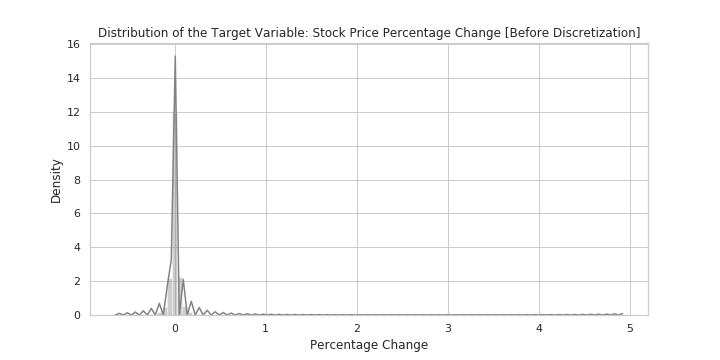
\includegraphics[width=\linewidth]{img/dist_target_nondisc.png}
		\caption{Distribution of the target variable before discretization}
		\label{fig:dist_target_nondisc}
	\end{figure}

	\subsubsection{Target Variable After Discretization}
		
	The normalized percentage changes were discretized into five bins of equal size, representing the five classes that are to be predicted in this project. Discretization into bins of equal size was used as discretization method to ensure balanced classes without having to over or undersample. Five bins were chosen to be able to distinguish between large, small and irrelevant percentage changes. The five classes correspond to large percentage decrease (\lstinline{lg_dec}), small percentage decrease (\lstinline{sm_dec}), no relevant change (\lstinline{same}), small percentage increase (\lstinline{sm_inc}) and large percentage increase (\lstinline{lg_inc}).
	
	Table ~\ref{table:stats_by_target} shows descriptive statistics for the percentage changes after discretization. This table basically illustrates what the classes used in this project actually represent. For instance, the class  \lstinline{lg_dec} represents any percentage change in the interval $[-0.9386, -0.0217]$. Here, $-0.9386$ represents $-93.86$ percent. Figure ~\ref{table:stats_by_target} shows the number of observations by training, validation and test data. The classes are very balanced, i.e. they occur similarly often, in the overall data as well as across the different data sets.
	
	\begin{table}[h!]
		\centering
		\caption{Descriptive statistics for percentage change by discretization level}
		\label{table:stats_by_target}
	
		\begin{tabular}{lrrrrrr}
			\toprule
			Disc. Level &  size &     min &     max &    mean &  median &     std \\
			\midrule
			lg\_dec &  8355 & -0.9386 & -0.0217 & -0.0681 & -0.0451 &  0.0687 \\
			sm\_dec &  8386 & -0.0217 & -0.0051 & -0.0121 & -0.0116 &  0.0047 \\
			same   &  8365 & -0.0051 &  0.0054 &  0.0002 &  0.0002 &  0.0030 \\
			sm\_inc &  8315 &  0.0054 &  0.0226 &  0.0126 &  0.0119 &  0.0048 \\
			lg\_inc &  8342 &  0.0227 &  4.9105 &  0.0736 &  0.0473 &  0.1166 \\
			\bottomrule
		\end{tabular}
	\end{table}%		


	\begin{figure}[h!]
	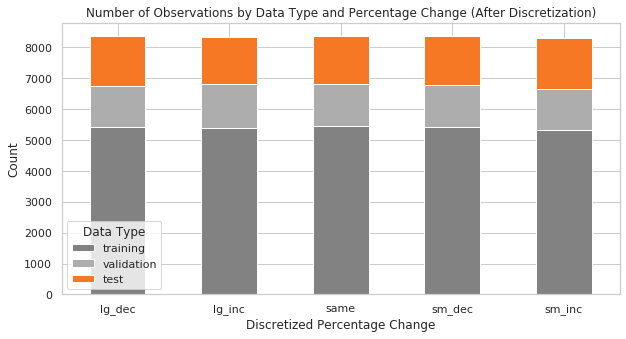
\includegraphics[width=\linewidth]{img/dist_target_disc.png}
	\caption{Distribution of the target variable after discretization}
	\label{fig:dist_target_disc}
	\end{figure}


	\subsubsection{Other}
	
	The distribution of the number of tokens per document is shown in figure ~\ref{fig:dist_num_tokens}. There are few documents with more than 10000 tokens. The largest 8-K filing has approximately 75000 tokens. Note that any filings with more than 1 Mio. characters have been filtered out before during pre-processing.
	
	The number of occurences of each 8-K events is displayed in figure ~\ref{fig:dist_8k_events}. Note that one 8-K filing can contain information about more than one event. Therefore, the total number of events is more than twice as large as the total number of 8-K filings. The five most frequent events are: 9.01 (financial statements and exhibits), 2.02 (results of operations and financial condition), 8.01 (other events), 7.01 (regulation FD disclosure) and 5.02 dDeparture of directors or certain officers; election of directors; appointment of certain officers; compensatory arrangements of certain officers).

	\begin{figure}[h!]
		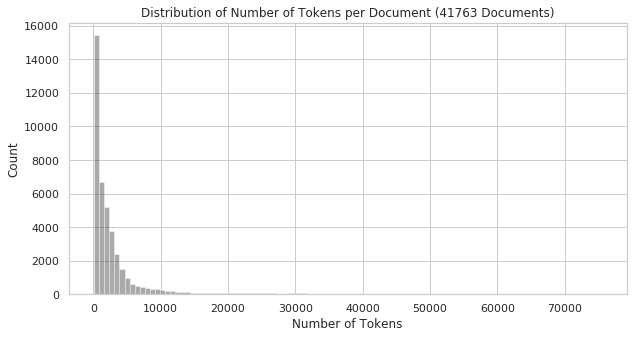
\includegraphics[width=\linewidth]{img/dist_num_tokens.png}
		\caption{Distribution of the number of tokens per document}
		\label{fig:dist_num_tokens}
	\end{figure}


	\begin{figure}[h!]
		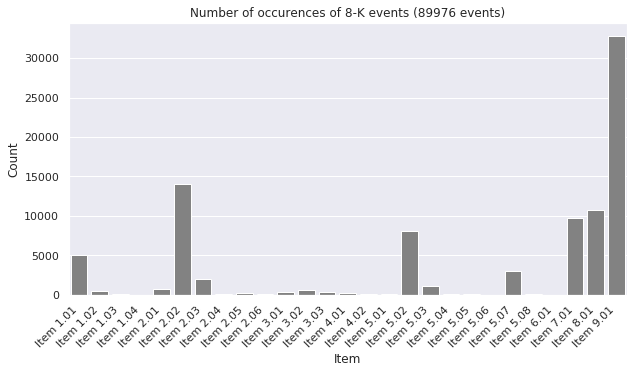
\includegraphics[width=\linewidth]{img/dist_8k_events.png}
		\caption{Number of occurences of 8-K events}
		\label{fig:dist_8k_events}
	\end{figure}


	\section{Method}
	
	\subsection{Training, Validation, Testing}
	
	The available data covers the complete year 2018 and the first quarter of 2019, i.e. five quarters in total. The four quarters of 2018 were used as training and validation data and the first quarter of 2019 was used as test data. The data for 2018 was split randomly into 80 percent training and 20 percent validation data. 
	
	The training data was used to train the models (with and without cross validation). In particular, cross validation with three folds based on the training data was used when doing grid search for hyperparameter optimization. For the baseline models, the full training data was used without cross validation. After training, all models were evaluated on the validation data. Based on the performance on the validation data, the best model was chosen. This model was then evaluated on the test data to obtain a generalization error and evaluate whether we could use the model in practice. 
	
	\subsection{Feature Pre-processing}
	
	%df_min, df_max%
	
	\subsection{Evaluation Metrics}
	
	For evaluating the results, confusion matrix, accuracy and class-wise precision are reported. Accuracy was used to determine the best model. When interpreting the performance of the best model on the test data, the focus was on class-wise precision, an important metric for considering potential trading strategies based on the model.
	
	Class-wise precision is computed for each class individually. For a given class c, the class-wise precision is defined as the number of observations of class c that were classified as class c (TP for true positive), divided by the number of any observations that were classified as class c, regardless of whether they are of class c or not (TP + FP for the sum of all true positives and false positives).
	
	\begin{align}
	\mathrm{precision}_c = \frac{TP_c}{FP_c + TP_c}
	\end{align}
	
	Using precision as prioritized evaluation metric for the final model reflects the assumptions that a) we want to avoid loosing money in a trade and that b) missing out on a good trade is acceptable. To explain this, it is best to consider an example. Assume that we take a long position whenever the model classifies a large stock price increase (\verb|lg_inc|), i.e. we buy stocks expecting that their stock price will increase. If the stock price decreases instead, we would loose money. To avoid this loss, we ideally want that among all cases where the model classifies a large increase (FP + TP), the stock price actually increases (TP). This means that we care about the precision. 

	
	\subsection{Loss Function}
	
	For multi-class classification problems, the softmax function is generally used as loss function (in neural networks and in gradient boosting trees). Hence, it is also used for this project. The loss functions used for GBDT and LSTM are generally the same but they differ slightly because in GBDT, each observation $i$ is weighted with $w_i$.
	
	\subsubsection{GBDT}
	
	The loss function used for CatBoost is called \lstinline{MultiClass} loss function and is essentially a weighted softmax function \cite{noauthor_multiclassification:_nodate}. It is computed as a scalar value across all observations and classes. The definition is as follows:
	
	\begin{align}
	L = \frac{\sum_{i = 1}^N w_i \log \left(\frac{\exp a_{i, t_i}}{\sum_{j = 0}^{M-1} \exp a_{i, j}}\right)}{\sum_{i = 1}^N w_i}, 
	\end{align}
	
	where $i = 1, ..., N$ is the index for the observation, $j = 0, ..., M-1$ is the index of the class, $a_{i, j}$ is the model output for observation $i$ and class $j$, $w_i$ is the weight assigned for observation $i$ during training, and $t_i$ is the index of the true class of observation $i$ so that $a_{i, t_i}$ is the model output for the true class of observation $i$.
	
	Essentially, the term in the parentheses is the softmax function, which returns a value between 0 and 1 for each observation $i$ to belong to its true class $t_i$. If the model performs well for observation $i$, then the softmax value will be large. For instance, if the value is 1, this means that according to the model, we have a probability of 1 that observation $i$ is from class $t_i$, i.e. from the true class of the observation. In other words, the model would perfectly identify the true class of observation $i$. Since the log is taken, and since $log(1)=0$, the loss incurred for this perfectly classified observation will be 0. If the softmax value is smaller than 1, the loss for an observation will be negative and will hence affect the training process.
		
	\subsubsection{LSTM}
	
	The loss function used for the LSTM is similar to the loss function from CatBoost. However, the observations $i$ are not weighted by any particular weights $w_i$. Essentially, a softmax function is used in the output layer so that the model directly outputs probabilities for each observation $i$ to belong to class $j$. Then, the loss function \lstinline{CategoricalCrossentropy} is used in \lstinline{TensorFlow} \cite{noauthor_module:_nodate}. For a multi-class problem, the categorical cross-entropy is defined as follows:
	
	\begin{align}
	L = \frac{\sum_{i = 1}^N \log \left(\frac{\exp a_{i, t_i}}{\sum_{j = 0}^{M-1} \exp a_{i, j}}\right)}{N}, 
	\end{align}
	
	where the notation is the same as in the loss function for GBDT. Note that in other notations this loss function usually has another sum over the classes along with an indicator function that is multiplied with the log (implying whether observation $i$ is from class $j$). However, here $a_{i, t_i}$ is defined as the model output for the true class of observation $i$ and hence the indicator function is not needed.
	

	% https://deepnotes.io/softmax-crossentropy
	

%	$$P(y = c | \textbf{x}) = \frac{\exp{z_c}}{\sum_{k = 1}^K \exp{z_k}}$$
	
	 %$\textbf{x}$ is a feature vector for one observation, $c$ is its corresponding class index, $K$ is the total number of classes, and $z_c$ is a real number given as output by the model. For instance, with a linear model, we might have $z_c = \textbf{x}^T\textbf{w}_c + b_c$. Basically, the model output $z_c$ is normalized by the softmax function to get a value in the interval from 0 to 1. This value is then interpreted as probability that observation $\textbf{x}$ corresponds to class $c$. A classification for observation $\textbf{x}$ can be obtained by taking $\underset{c}{\mathrm{argmax}} \ P(y = c | \textbf{x})$.
	
	
	\subsection{Hyperparameter Tuning}
	
	
	\subsubsection{Interpretation of Best Model}
	
	Visualization, Backtesting
	
	In addition to reporting the evaluation metrics numerically, they are also visualized by certain categorical variables (e.g. industry of the company, event of the 8-K filings, location of the company) in order to identify issues as well as future potentials of the models. 
	
	\section{Results}

	\section{Discussion}
	
	\section{Conclusion}
	
	\section{References}
	
\printbibliography
\end{document}